Deep learning applications in recent years have come to require rapidly growing amounts of labeled training data.
Often, accuracies can be boosted by adding data as much as by spending years on algorithmic development.
For example, on the VOC07 benchmark, Faster-RCNN~\cite{FasterRCNN} with VGG-16 was able to eliminate 27.5\% of errors in the much older R-CNN~\cite{RCNN} backed by an equally old neural network architecture (mAP improved from 58.5 to 69.9). 
However, simply by including additional data from VOC12 and COCO, 29.5\% of the remaining error was eliminated (mAP improved from 69.9 to 78.8). 

\begin{figure}[h]
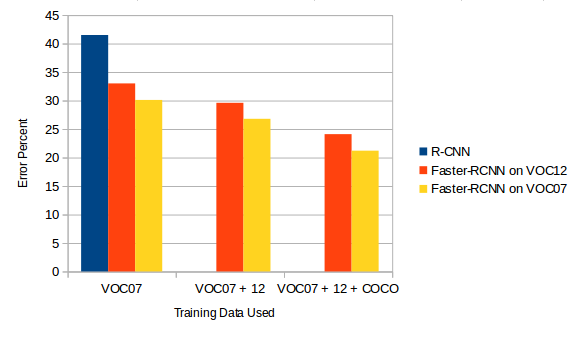
\includegraphics[width=14cm]{figs/data_vs_error.png}
\centering
\caption{Improvement of error as data increases, compared to error improvements due to algorithm improvements. 
As we can see by comparing the drop from RCNN to Faster-RCNN on VOC07 only, and the drop from adding training data to Faster-RCNN, increasing data contributes significantly to error reduction.}
\end{figure}

Therefore, for real-world application development, data can be cheaper and more effective than scientists. 
While many existing tools support image classification -- it is even built into Amazon Mechanical Turk (MTurk) -- and some tools support bounding box labeling in images, few tools exist for frame-by-frame labeling in videos. 
VATIC~\cite{Vatic} stands out as being one of the best, as not only does it make high quality annotations one of its main goals, but also cost and scalability. 

My work borrows and improves upon many concepts and results from VATIC's user studies, but I focus on an additional goal that is extremely important in creating datasets for real applications. That goal is researcher happiness.
Although VATIC extensively tested its ``User Interfaces'', I argue in chapter~\ref{chap:experimenter} that both the annotators and the experimenters are users, and the interfaces should be smooth for both when creating a tool.

Then, in chapter~\ref{chap:annotator}, I discuss my take on VATIC's User Interface principles for the annotator, and improvements upon them.

I also release all related code for BeaverDam, my video labeling platform, on Github.\footnote{http://github.com/antingshen/beaverdam}

\section*{Related Work}
\label{sec:related}

Static image annotators

Youtube video dataset

Vatic, LabelMe, etc

Things other people cite

KITTI, Berkeley group, samasource
